\chapter{Research}

\section{Introduction}

The outline of this research report is as follows: First we explain the problem domain, and provide an analysis. Secondly we state our project's requirements. Based on these requirements we formulate a research question that embodies our main objectives, followed by a technical analysis. The final part of this research report provides us with the optimal solution for our problem.


\section{Problem Domain} % (fold)
\label{sec:problem_domain}

% section problem_domain (end)

Within the following section we will describe and analyse what our problem domain is, identify the stakeholders, construct the scope and objectives, and summarize our interview we conducted from the Library's Head of Education Support.

\subsection{Domain Description} % (fold)
\label{sub:problem_description}

The goal of this project is the creation and implementation of a prototype for a `Virtual Assistant', which helps students and researchers to write a report, thesis or dissertation. This Virtual Assistant should provide its users with the ability to choose a layout template, allow for scheduling and feedback, and give suggestions or tips to users about how to write a report, thesis or dissertation.
This project should entail either native desktop software, a web application, or a mobile application. The final product should be released as open source software.

\subsection{Domain analysis} % (fold)

One of the key aspects that need to be well-researched for our project is our domain analysis. The domain analysis basically illustrates all the different types of roles involved with the problem domain (i.e. the stakeholders), and what their interests are. First we list all the stakeholders involved with our domain, secondly we define our scope, and finally we summarize a set of interviews we have conducted with people that embody relevant roles.

\subsubsection{Stakeholders} % (fold)

Below we identify the different stakeholders, which roles they can take, and what their main interests are within our problem domain.

\paragraph{Client: TU Delft Library} The TU Delft Library is the entity that requested this project, and is therefor our client. They expect a prototype of a product that meets their requirements.

\paragraph{Users: Students and Researchers} The use of this product is aimed at students, and researchers, which makes them a subset of our users. They want a product that is easy to use and helps them with writing a report/thesis/dissertation.

\paragraph{Users: Reviewers} The use of this product is also aimed at reviewers, which makes the complementary subset of our users. They also want a product that is easy to use and facilitates them in reviewing a report/thesis/dissertation.

\paragraph{Contributors: Open Source Developers} Our client requested that our final version be released as an open source project. This means that at some point in the future other developers are going to improve upon our product. With this in mind, we have to introduce some design ideals and constraints that will make it easier for them to add code in the future.

\subsubsection{Scope \& Objectives}

The scope of our domain is set for the use-case of students who are writing a Bachelor project final report. One obvious reason for this scope is that this project is also a Bachelor final project, which will also include the process of writing a final report. This means that we will have affinity with the scope, which should imply an advantage within our design. Another reason is that there are plainly too many different cases and subjects within our problem domain to serve all of them accordingly within our deadline.
Our main objective is the creation of an online environment that acts as a support for students who are writing a report/thesis/dissertation. It should provide the students with suggestions, tips, sources and other relevant information. It should provide a platform where there is an interaction between students and their peers or superiors (in this case a teacher, coach or supervisor), and where they can exchange feedback towards each other.

\subsubsection{Interview result analysis} % (fold)

The most challenging part in this project is understanding how we can provide suggestions, tips, sources and other relevant information to students. In order to get a more detailed comprehension of this part within our problem domain, we conducted an interview with Nicole Will. Nicole works for the TU Delft Library as the Head of Education Support, and is also involved with the TULib website, which is an informative website about finding and using scientific information.
We wanted to know what the most valuable pieces of information were that we could provide students with when they write a report. She claimed there were three important parts that we should include, being the module on how to cite\cite{tulib:howtocite}, how to make a reference list, and how to use the APA\cite{tulib:apa} style for your references.
Other than these she also found it useful to provide the students with information on how to find information and articles, how to check for relevance and reliability of sources and what plagiarism is and how to avoid it.

\subsection{Research Question}

The context of this project is to build an application that acts as a virtual assistant to help Bachelor students write their article/report in a correct manner. In order to design a robust and reliable software application, we first need to formulate a research question to do the technical research and to come up with a feasible and optimal solution for developing a prototype application.\\\\

During the first meeting that involved both our client and coach, the latter has persuaded us to develop a web application. Throughout the rest of this research report we will primarily assume that a web application is most likely the best choice of platform, whereas the research itself is intended to find out whether this assumption is correct, and if so, why it would be an ideal choice. \\\\

The main research question is formulated as follows: `How do we build a reliable and robust web application prototype that is able to assist students in writing an article or report, and is also able to guide them in such a way that they are able to write an article or report in a correct and efficient manner within the time constraint that is given to them? '

\subsection{Project Requirement}

The requirements provide the backbone to a project. They are confirmed in accordance with our client and our coach. It is imperative that these requirements are met at the end of the implementation.

\subsection{Functional Requirements} % (fold)
\label{sub:functional_requirement}

Below is a list of functional requirements that the application should meet:

\begin{enumerate}
	\item Multiple Users: Each project created by one user can be joined by multiple other users, where none or more joining participants can be attributed owner privilege. The creator of the project will receive owner privilege by standard. The application should also facilitate reviews from supervisors or other members.
	\item Template: The application will provide several templates for the user, or the user can upload his of her own template
	\item Schedule: There has to be a module in which the users can schedule their writing progress according to their chosen template. (In terms of sections such as introduction etc.)
	\item Propose Suggestions/Tips: The system should be able to suggest tips and information to the user on how to write specific sections.
	\item Send/Receive Feedback: The application should facilitate feedback on a report written by a student from a reviewer.
	\item Done/Discard: For each suggestion or piece of feedback, the student can choose to check it off as `Done' or `Discarded'. When a user has checked `Done' or `Discarded' on the suggestion or piece of feedback, both the system and all other users should be notified. 
	\item Upload Document: Ability to upload the document into the application.
	\item Built-in Chat mechanism: To display the feedback from a reviewer and keep track of the conversations. 
	\item Versioning : Keep track of the versions of publications that a user has uploaded.
	\item Logging : Save the user's records in a separate log file for usage analytics.
\end{enumerate}

% subsection functional_requirement (end)
\subsection{Technical Requirements} % (fold)
\label{sub:technical_requirements}

Besides the functional requirements, which illustrate how the system should work in usage, there are also some technical requirements that illustrate how the system should be built. These technical requirements are listed below:

\begin{enumerate}
	\item Provide Mobile Support for Android/IOS
	\item Campus ID authentication: allow login with TUDelft netID
	\item Released as Open Source
 	\item System should be fully tested 
\end{enumerate}

% subsection technical_requirements (end)
\subsection{Usability Requirements} % (fold)

Finally there are also some usability requirements that should be met in order to guarantee a user-friendly application:

\label{sub:usability_requirements}
\begin{enumerate}
	\item The application must be fully functional on modern web browsers
	\item Efficient in use: System must facilitate efficiency of use for the user by providing information on the fly for the context
	\item Intuitiveness: User Interface must be intuitive and easy to use
\end{enumerate}
% subsection usability_requirements (end)
\newpage
\subsection{Technical Analysis} % (fold)

Now that the requirements are set, and our research question has been formulated, we know what type of features we are looking for in a technical setting. In this section we illustrate our findings, and justify our choices in terms of tools deployment, architecture design and system components.

\subsection{Why a web application?}
One of the main ideas that have been advised to us by our coach is the creation of a web application for our project. The justification for this is ease of usability and compatibility across several platforms. Web applications are also exempted from platform-specific updates, whereas now one single update on the web application immediately reaches all of our users at once. When a web application is used, users can access the exact same content from different computers or mobile devices.
\newpage
\subsection{Objective}
There are various frameworks available for the implementation of a web application. The choice of a specific framework usually depends on the context and objectives of the project itself. Our current project entails the development of a prototype within a time constraint of 11 to 12 weeks, which persuaded us to use a full stack framework. If we would use a full stack framework, we should be able to focus primarily on techniques that allow us to perform rapid prototyping, generate quality code and provide good documentation all of which meet the clients requirements. The following features should facilitate reaching our objectives during the development phase.

\begin{enumerate}
	\item \textbf{a Full-Stack framework}: A framework that already contains all the basic utilities to create and run an application, with the option to connect or import external entities too.
	\item \textbf{Rapid Prototyping}: Allows us to convert the clients requirements into a prototype in a fast way so it can be immediately reviewed and refined for the next prototype.
	\item \textbf{Scalability}: The ability of a system, network, or process to handle a growing amount of work in a capable manner or its ability to be enlarged to accommodate that growth.\cite{wiki:scalability}
	\item \textbf{Reliablity}: The ability of a system to function under predefined conditions.
\end{enumerate}
\subsection{Project Development Methodology} % (fold)

For our project development methodology we chose the agile Scrum methodology. This means that we will have weekly sprints (iterations within a fixed amount of time) in which a predefined set of items, taken from a product backlog\footnote{The agile product backlog in Scrum is a prioritized features list, containing short descriptions of all functionality desired in the product.\cite{backlog} }, are to be implemented. Each week we show our client what we achieved, and we discuss possible changes (within the requirements that have been agreed upon). The Scrum method gives developers an advantage over sequential methodologies such as the waterfall model or the V-model, because when changes have to be made to either pieces of code, features or even requirements, the sequential methodologies force the developers to revise (or even redo) everything that happened after the point where they were processed within the implementation. These sort of changes are more manageable within iterative methodologies such as Scrum. Scrum also allows developers to uncover designing constraints that may not have been obvious at the start of the implementation by giving them the opportunity to pivot after every sprint. \\\\
Given these advantages, the use of the Scrum method should be the most adequate for our project. When using Scrum, some roles and conventions have to be attributed, which are listed below:

\begin{enumerate}
	\item \textbf{Roles}
		\begin{itemize}
			\item Product Owner/Dev Team: Arnaud Hambenne
			\item Scrum master/Dev Team: Soheil Jahanshahi
			\item Client: TU Delft Library (Babak Dehghenpour, Nicoleta Nastase)
			\item Coach: Alberto Bacchelli
		\end{itemize}
		\newpage
	\item \textbf{Conventions}	
\begin{itemize}
		\item Sprint duration: One week.
		\item Sprint Planning meeting: A weekly meeting that is used to prioritize the selected features for each sprint. 
		\item Sprint reflection report: A weekly evaluation where the estimated effort is compared to the actual effort that was needed to implement the chosen features, and where possible issues are documented. The evaluation takes place at the end of each Sprint.
		\item Daily Scrum meeting: A daily meeting between the developers which takes about 15 minutes.
		\item Sprint review meeting: A weekly meeting of about 15-20 minutes with the clients, in order to receive their feedback on the implemented features.
\end{itemize}
\end{enumerate}

\subsubsection{Definition of Done} 
In order to be sure that every component functions correctly, we narrow down the definition we use for the word `done'. When we say a function or the application is `done' we mean that it is: 

\begin{itemize}
	\item	Implemented (the code has been written)
	\item	Unit tested (JUnit test cases)
	\item 	Integrated
	\item 	Integration tested
	\item 	Documented (the change has been documented)
\end{itemize} 

\subsection{Architectural Model : MVC}
Having a design pattern is important when you want to write re-usable and maintainable code.
For the `Virtual Assistant' application we decided that it is best to divide the application into three interconnected parts which separate the internal representation of data from information that is presented to the users\cite{wiki:mvc}. This type of designpattern is called the MVC pattern. MVC stands for the three components that make up the pattern, the Model, the View and the Controller.
\begin{figure}[h]
\centering
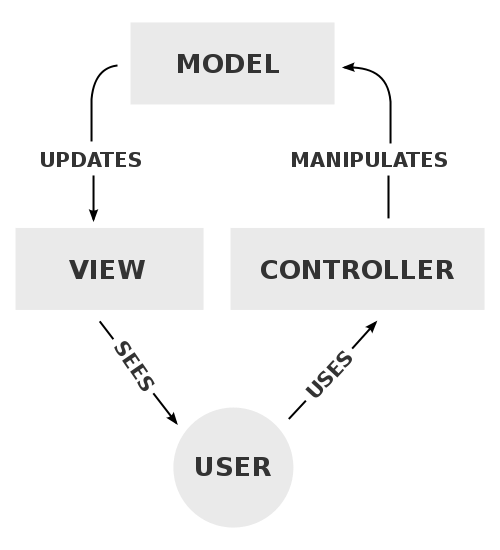
\includegraphics[scale=0.3]{./img/MVC.png}
\caption{\small{The Model, View and Controller, interconnected by directed edges}}
\label{mvc}
	
\end{figure}

As shown in fig \ref{mvc}, the MVC separates the application into a front end, the View, and a back end, the Model and Controller. The Controller provides the link between both the View and the Model, which makes it act as the brain of the application. The Controller decides what the user input was and how the Model needs to change as a result of this input\cite{codinghorror}. The Controller then responds back to the user by calling the resulting View.

\subsection{Choice of framework}
In order to be able to choose a suitable web application framework, we have defined some  constraints for ourselves that we can use to benchmark various popular existing frameworks. Our first criteria was choosing a framework which is based on either Java, Scala or Javascript. With this in mind, we have narrowed our choices down to four popular frameworks such as \href{https://grails.org/}{Grails}, \href{https://vaadin.com/home}{Vaadin}, \href{https://www.playframework.com/}{Play!} and \href{http://projects.spring.io/spring-framework/}{Spring}. Finally we were able to boil down our choice to either the Spring framework or the Play! framework.
\subsubsection{Benchmarking}
 The table below lists the comparison of these two frameworks within the constraints that we have defined:\\

\begin{figure}[h]
\centering
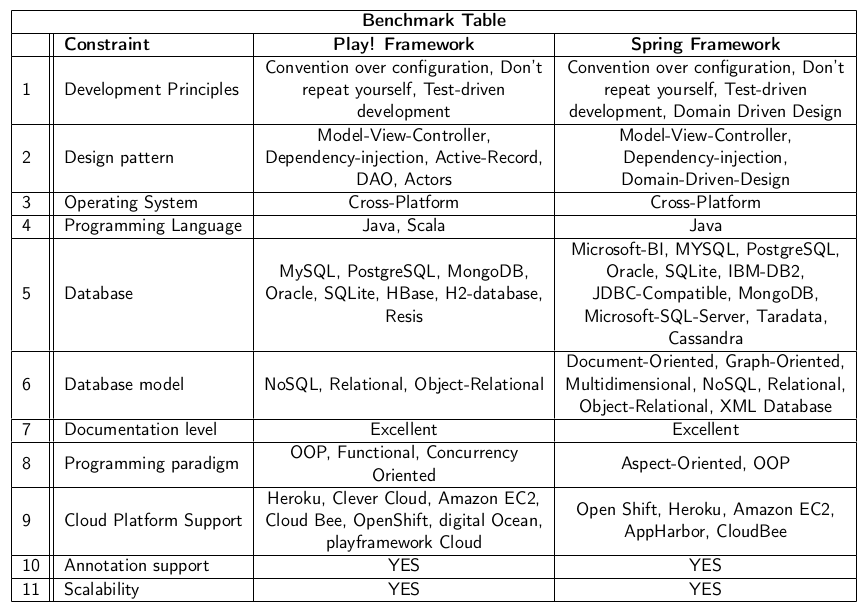
\includegraphics[scale=0.5]{./img/benchmark.png}	
\end{figure}

% \begin{center}
% \begin{tabular}{ |l||l| C{6cm} | C{6cm} |  }
%  \hline
%  \multicolumn{4}{|c|}{\textbf{Benchmark Table}} \\
%  \hline
%  ~ & \textbf{Constraint} & \textbf{Play! Framework} & \textbf{Spring Framework}\\
%  \hline
%  1 & Development Principles & Convention over configuration, Don't repeat yourself, Test-driven development & Convention over configuration, Don't repeat yourself, Test-driven development, Domain Driven Design \\
%  \hline
%  2 & Design pattern & Model-View-Controller, Dependency-injection, Active-Record, DAO, Actors & Model-View-Controller, Dependency-injection, Domain-Driven-Design \\
%  \hline
%  3 & Operating System & Cross-Platform & Cross-Platform \\
%  \hline
%  4 & Programming Language & Java, Scala & Java \\
%  \hline
%  5 & Database & MySQL, PostgreSQL, MongoDB, Oracle, SQLite, HBase, H2-database, Resis & Microsoft-BI, MYSQL, PostgreSQL, Oracle, SQLite, IBM-DB2, JDBC-Compatible, MongoDB, Microsoft-SQL-Server, Taradata, Cassandra \\
%  \hline
%  6 & Database model & NoSQL, Relational, Object-Relational & Document-Oriented, Graph-Oriented, Multidimensional, NoSQL, Relational, Object-Relational, XML Database \\
%  \hline
%  7 & Documentation level & Excellent&Excellent \\
%  \hline
%  8 & Programming paradigm & OOP, Functional, Concurrency Oriented&Aspect-Oriented, OOP \\
%  \hline
%  9 & Cloud Platform Support & Heroku, Clever Cloud, Amazon EC2, Cloud Bee, OpenShift, digital Ocean, playframework Cloud & Open Shift, Heroku, Amazon EC2, AppHarbor, CloudBee \\
%  \hline
%  10 & Annotation support & YES & YES \\
%  \hline
%  11 & Scalability & YES & YES \\
%  \hline
% \end{tabular}
% \end{center}

The result of this benchmark shows us that the differences between these two frameworks are fairly minimal. We decided to use the Play!Framework for this project.
\newpage

\subsection{Play! Framework}
  One of the main reasons we selected the Play! Framework is because this framework has been proven in production. For example the LinkedIn web application has been developed using the Play! Framework. The following figure\ref{play} illustrates an overview of the Play! Framework.\\
\begin{figure}[h!]
\centering
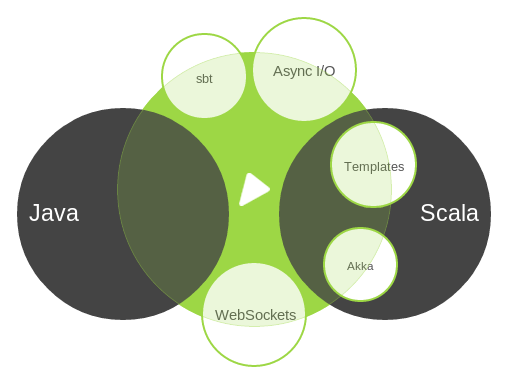
\includegraphics[scale=0.5]{./img/play.png}
\caption{\small{The main attributes and features of the Play! Framework}}
\label{play}
\end{figure}
 
 
The Play! Framework offers excellent documentation\cite{playDoc} that can help us get familiar with the Play! environment. First of all, it is an open source application that has an amazing error handling because of the fact that everything is compiled and built on the fly. This makes it easier for developers to detect bugs and can dramatically improve the developer's productivity to make changes. By reloading the browser, you can immediately see the changes you just made, which makes it perfect for fast prototyping within our project. Moreover, Play! supports both the Scala and Java languages, it comes with a Scala template that allows you to write dynamic code within an HTML body, and it also comes with pre-configured testing support. This last one is particularly important because that means we do not need to worry about adding Junit dependencies to the build file. \\\\
Play! also offers the use of the EBean server interface which is very handy for fetching and saving beans to a particular DataSource. It can make reactive applications simpler because Play! is built on \href{http://netty.io/}{Netty}, which means it supports non-blocking I/O.\footnote{ non-blocking I/O is a form of input/output processing that permits other processing to continue before the transmission has finished.} This will enable our web application to make remote calls inexpensively which is crucial for high performance web applications.





